\documentclass[10pt,conference]{IEEEtran}
\IEEEoverridecommandlockouts
\IEEEpubid{\makebox[\columnwidth]{978-1-7281-5127-4/20/\$31.00~\copyright{}2020 IEEE \hfill} \hspace{\columnsep}\makebox[\columnwidth]{ }}
\usepackage{cite}
\usepackage{amsmath,amssymb,amsfonts}
\usepackage{algorithmic}
\usepackage{graphicx}
\usepackage{textcomp}
\usepackage{xcolor}
\usepackage{url}

\newcommand{\notedm}[1]{\textcolor{red}{Daniele: #1}}
\newcommand{\notect}[1]{\textcolor{violet}{Cedric: #1}}
\newcommand{\notedb}[1]{\textcolor{gray}{Davaa: #1}}


\def\BibTeX{{\rm B\kern-.05em{\sc i\kern-.025em b}\kern-.08em
    T\kern-.1667em\lower.7ex\hbox{E}\kern-.125emX}}
\begin{document}


\title{FogGuru: a Fog Computing platform based on Apache Flink\\}

\author{\IEEEauthorblockN{Davaadorj Battulga}
\IEEEauthorblockA{\textit{U-Hopper, Univ Rennes, Inria, CNRS, IRISA}\\
davaadorj.battulga@u-hopper.com}
\and

\IEEEauthorblockN{Daniele Miorandi}
\IEEEauthorblockA{\textit{U-Hopper}\\
daniele.miorandi@u-hopper.com}
\and

\IEEEauthorblockN{C\'{e}dric Tedeschi}
\IEEEauthorblockA{\textit{Univ Rennes, Inria, CNRS, IRISA}\\
cedric.tedeschi@inria.fr}
}

\maketitle

\begin{abstract}
Fog computing infrastructure aims to offload computing resources from cloud providers by placing edge devices closer to end-users and/or data sources. Systems and methods for developing and deploying an application in Fog nodes are still in their infancy. In this work, we present FogGuru, a fog computing platform meant to facilitate application deployment in Fog environments. FogGuru builds upon the stream processing paradigm for fog applications design; its implementation makes use of the open-source Apache Flink stream processing engine. The demo will showcase a Fog-based traffic analytics application deployed using FogGuru and running on a fog node, composed of a cluster of five Raspberry Pis.
 % (SPE) . SPEs are well suited in Fog computing platform based on their extensive features. The proposed platform was implemented using container orchestration and demonstrated on a cluster of resource-constrained devices.
\end{abstract}


\begin{IEEEkeywords}
Fog Computing, Edge Computing, Apache Flink
\end{IEEEkeywords}


%%%%%%%%%%%% Introduction %%%%%%%%%%%%%%%%
\section{Introduction}
\label{sec:introduction}
Fog Computing is an architectural approach for building computing infrastructure
meant to best support Internet-of-Things (IoT) applications and services. The
main idea behind fog computing is to enhance the performance of traditional
cloud computing applications by deploying computing
resources closer to end-users and data sources. Potential benefits include
reduced latency, bandwidth optimization, privacy and security, lower energy
consumption, and reduced dependency on
cloud providers. According to the OpenFog reference
architecture~\cite{openfogRA}, the key technical challenges in the maturation of
Fog Computing are scalability, autonomy, and programmability. Fog Computing
could enable highly adaptive deployments of services, including support for
programming at the software and hardware layers. 

A challenge stands in the fact that Fog Computing platforms will include both
computing resources at the edge and in more traditional Clouds. Operating a Fog
that gathers heterogeneous, geo-distributed nodes has been only very recently
addressed~\cite{fogdeploy} and is still a largely open problem. This work focus
on Fog nodes located at the edge of the network.

Re-tasking a fog node or cluster of nodes for accommodating operational dynamics
addressing rapidly changing requirements can be automated. However, this is
hindered by the lack of common models for programming fog nodes; as of today,
most fog deployments require a lot of manual intervention and use solutions for
specific use cases.

%\notedb{The problem is that Fog lacks programmability, there are a number of
%fog deployments, but they all require developers to have deep tech knowledge
%and designed for only one specific use case. What's a good way to express
%this?}

In this work, we aimed to design and develop a Fog platform, called FogGuru, for facilitating the development and deployment of Fog applications. Our approach is based upon the usage of a stream processing architecture for elaborating data from the IoT tier on the fog node (including operations such as aggregation and filtering). The prototype we built makes use of the real-time Stream Processing Engine (SPE) Apache Flink, which is provided as an image ready to be deployed on resource-constrained devices. We further provide support for automating the service deployment procedure (on both single nodes as well as clusters) and demonstrate its usage on a traffic analysis scenario.

The rest of the paper is organized as follows. Section II
presents the platform design and discusses some technology choices we made. Section III describes the prototype implementation. Section IV presents the actual demonstrator that will be showcased. Finally, conclusion and future work are presented in Section V.



%%%%%%%%%%%% Design and Technology %%%%%%%%%%%%%%%%
\section{Design and Technology}
\label{sec:Technology and Design}
\subsection{Hardware stack}
In principle, any device with computing, storage, and network connectivity could act as a fog node~\cite{ciscoFog}. Additionally, fog nodes should be able to be distributed geographically, to cope with different network types, to be cheap and easy to replicate. We chose to work with Raspberry Pi 3b+ (Quad-core 64-bit ARM processor, 1GB of RAM, 32GB of storage) single-board computers as standard devices. However, as such devices are rather limited in terms of processing capabilities (mostly related to the little amount of RAM available), we decide to build a small cluster of five Raspberry Pi 3b+, and use such cluster as fog node hardware platform. In Figure~\ref{fig:fridge} we present two images of the cluster, which we refer to as 'fridge'.
 % (Quad-core 64-bit ARM processor, 1GB of RAM, 32GB of storage) single-board computers as a cluster of hardware device \notedb{fig or pic of HW setup maybe}. We used D-Link DWR-921 router (with OpenWRT installed) as Wi-Fi Access Point for the clusters.
% }
\begin{figure}[htbp]
\centerline{
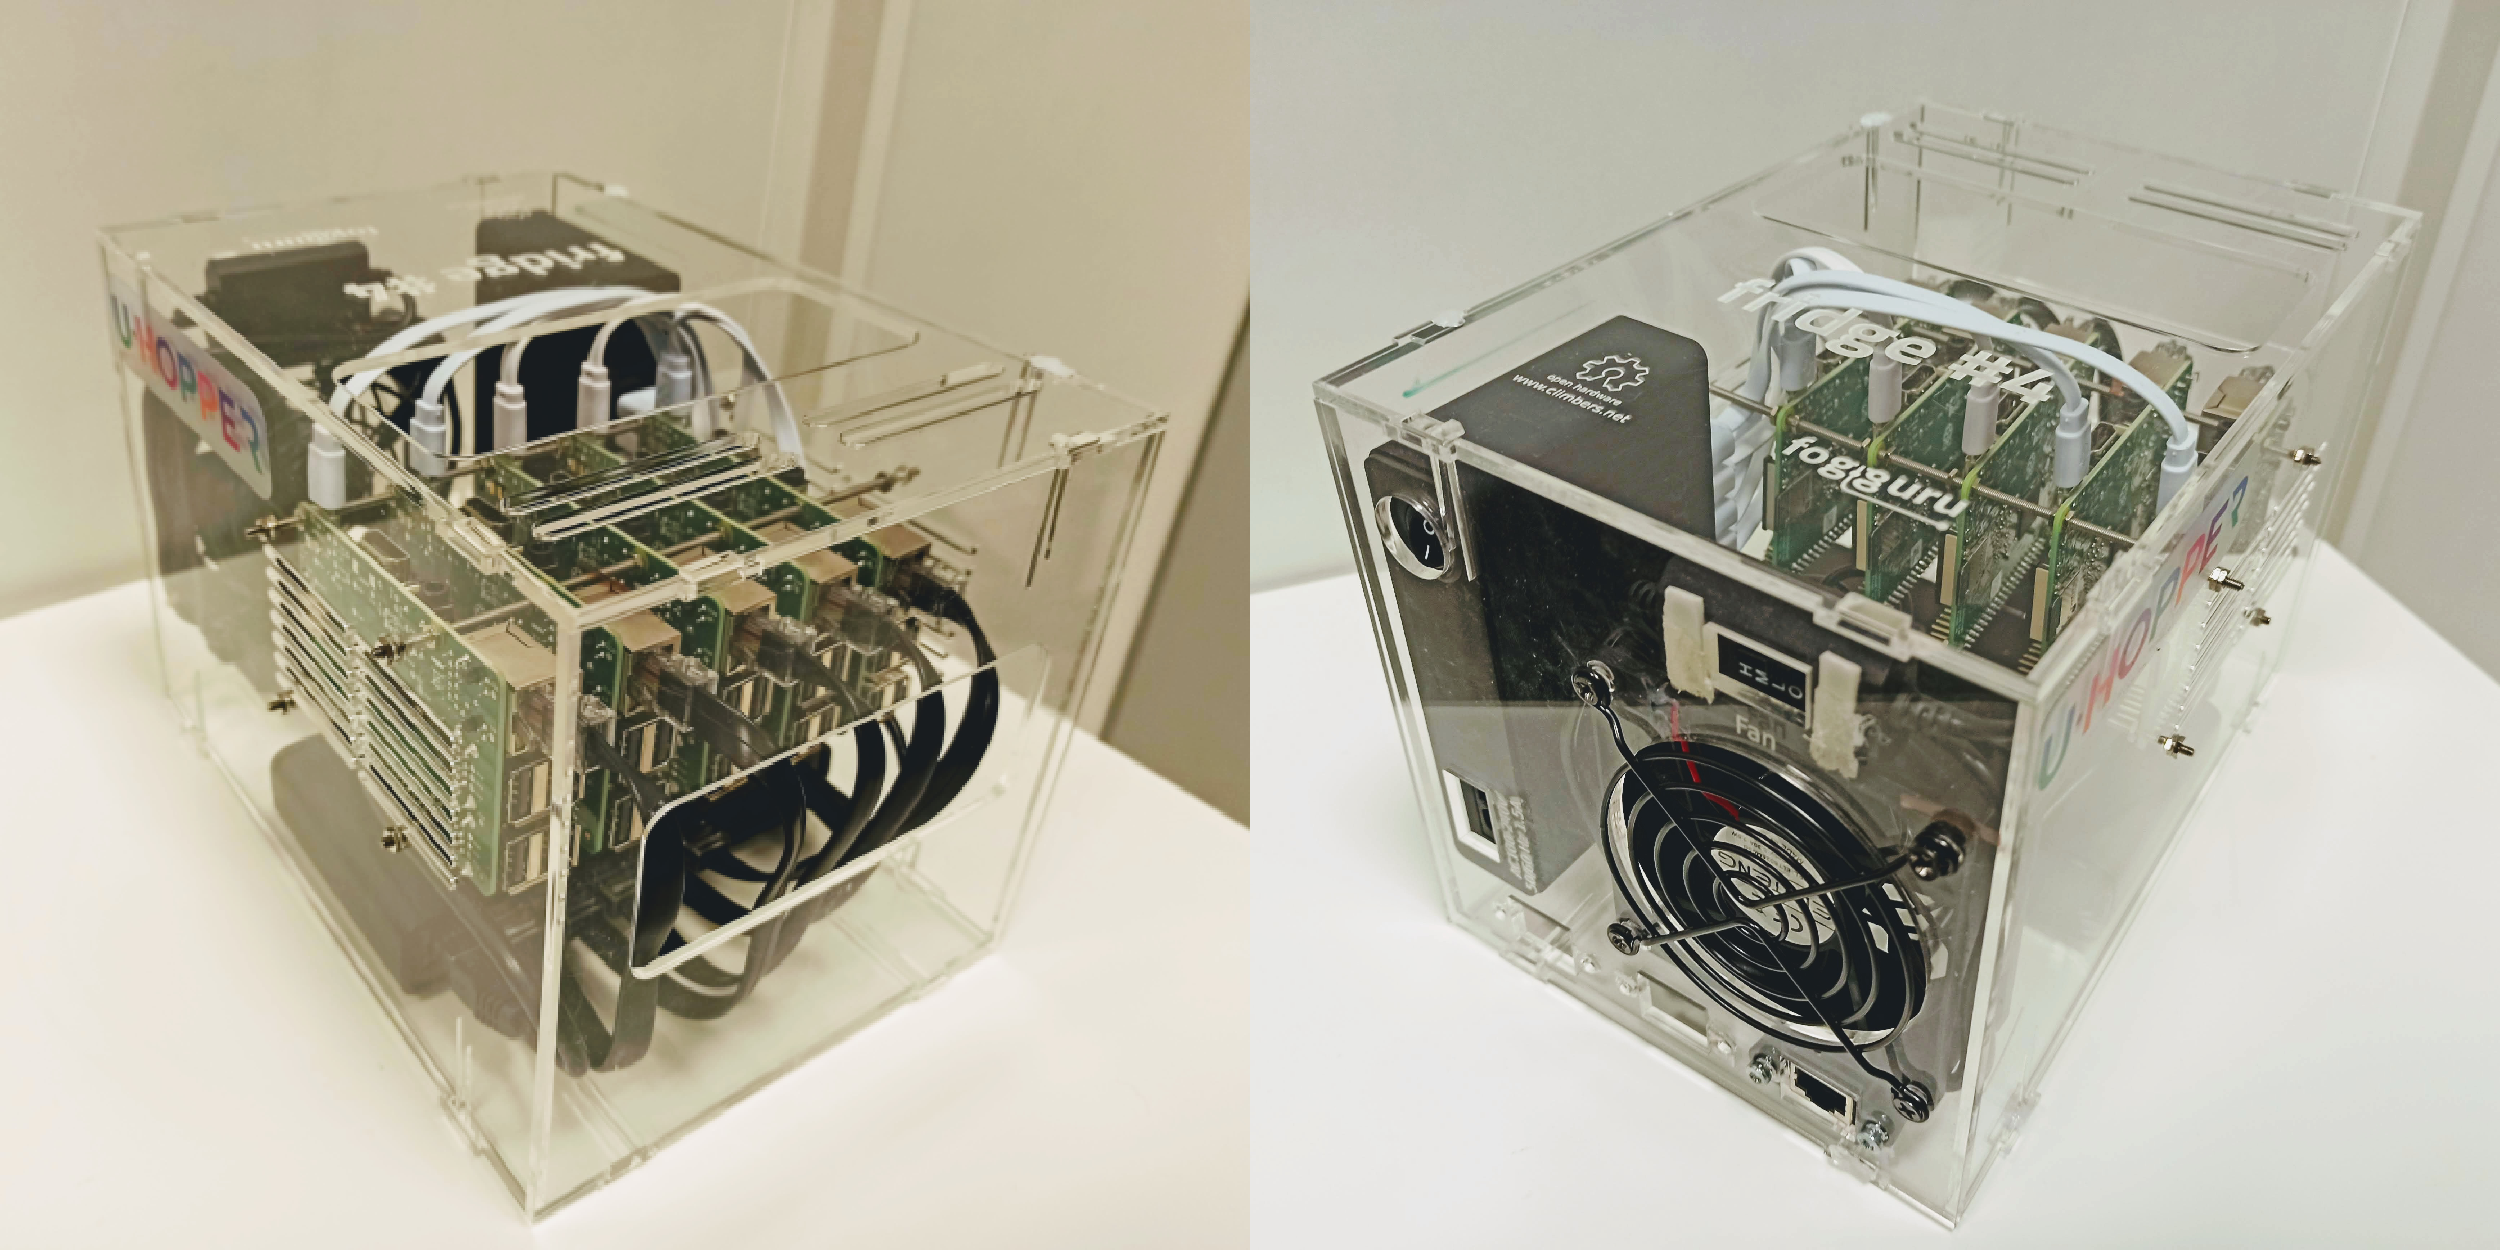
\includegraphics[width=1\linewidth]{figures/fog_pic.pdf}}
\caption{The FogGuru hardware platform (cluster of 5 Raspberry Pi 3b+), commonly referred to as 'fridge'.}
\label{fig:fridge}
\end{figure}


\subsection{Platform architecture}
The FogGuru platform high-level architecture is represented in Figure~\ref{fig:node-arch}. It is consistent with standard architectures in edge/fog computing (see~\cite{de2018distributed}) and in data processing pipelines~\cite{ismail2019manufacturing}. Data from the IoT tier gets ingested through a suitable queuing system, from where it is fetched to be (stream-)processed. Intermediate results may be fed back to the message queueing system and/or stored persistently, depending on the expected usage. Processed data (represented as a stream) is pushed to the cloud tier for further aggregation/analysis. The operations of the stream processing engine are monitored, and relevant log data (or basic analytics) are also pushed to the cloud tier in batches.
% indicated the key components in real-time data processing architecture. And they can be simplified, as shown in Figure~\ref{fig:node-arch}.

\begin{figure}[htbp]
\centerline{
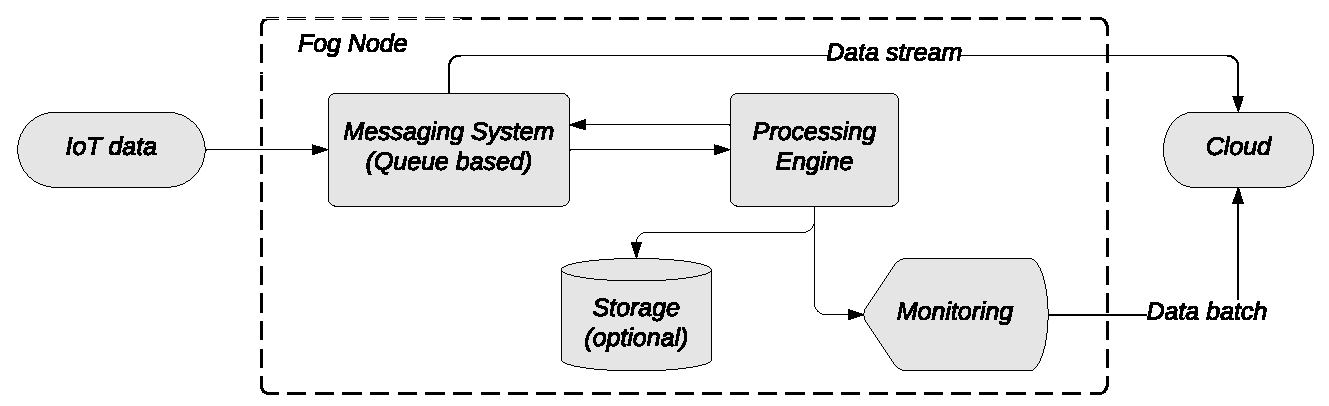
\includegraphics[width=1\linewidth]{figures/fog_components.pdf}}
\caption{The FogGuru platform architecture.}
\label{fig:node-arch}
\end{figure}

The choice of appropriate technologies/frameworks for implementing such an architecture plays a critical role. Here is a brief description of our design choices.
% Choosing a suitable software stack for the resource-constrained environment is crucial for fog application deployment.
\paragraph*{Messaging System}
Message Queue Telemetry Transport (MQTT) is a lightweight publish-subscribe network protocol widely used in IoT applications, and better suited for fog applications than more powerful (but resource-hungry) cloud frameworks (such as, e.g., Apache Kafka). We decided to use the open-source Mosquitto\footnote{https://mosquitto.org/} MQTT broker as our message handler.

\paragraph*{Processing}
Stream Processing Engines (SPEs) represent a good paradigm for Fog computing applications because of their extensive set of features, including support for event-driven, data pipeline, and data analytics applications. Constrained resources is also here an aspect to cater for; the literature includes surveys on how various SPEs perform in a fog environments~\cite{lee2017data,zeuch2019analyzing}. We decided to use Apache Flink\footnote{https://flink.apache.org/} as our SPE of choice. Apache Flink is a distributed, open-source, stream processor with intuitive and expressive APIs to implement stateful stream processing applications.

\paragraph*{Monitoring}
We used Prometheus\footnote{https://prometheus.io/} and Grafana\footnote{https://grafana.com/} for computing real-time performance indicators based on Apache Flink metrics APIs.
% as a time series Database for recording real-time metrics.
 % and Grafana as the web interface for analysis and visualization./notedm{remove reference to Grafana and focus on storage here, for the monitoring part leave it empty (we don't have it actually..)}

\paragraph*{Containerization}
Using container orchestration is mandatory for deploying fog applications at scale. It packages software components and their dependencies and deploys them in a standardized way. There are studies about performance evaluation of container orchestrators in Fog environment~\cite{hoque2017towards}. We used the Docker\footnote{https://www.docker.com/} ecosystem for its portable deployment.



%%%%%%%%%%%% Implementation %%%%%%%%%%%%%%%%
\section{Implementation}
\label{sec:implementation}
The resulting FogGuru deployment diagram is presented in Figure~\ref{fig:deployment}. It shows which components got deployed on which node, their roles and interfaces. To make it run, three main challenges had to be overcome.

\paragraph*{Creating the swarm nodes}
Docker Swarm can run on multiple resource-constrained devices such as Raspberry Pi. Using Docker CLI commands, it is possible to create cluster nodes. In our case, one node functions as a Swarm Manager node, others as Workers. The configuration deployed consists of 5 Raspberry Pis, interlinked locally with a docker swarm network.

\paragraph*{Getting Apache Flink to run on Raspberry Pi}
Apache Flink runtime consists of 2 types of processes: At least one Job Manager coordinates the distributed execution and Task Managers (workers) execute tasks and exchange data streams. The design is to run Job and Task managers on different swarm cluster nodes. To run Flink on Raspberry Pi, we configured the Job Manager heap-memory size to 512MB, and the Task Manager heap memory size to 256MB. Also, we enabled Flink's built-in monitoring and metrics system to allow developers to monitor their Flink jobs. Flink Metrics were queried via REST API, which used with Prometheus and Grafana for monitoring and visualizing.

We used dockers buildx feature to create custom Apache Flink docker image for ARMv7 processor and hosted the image on DockerHub public repository\footnote{https://hub.docker.com/repository/docker/digitaljazz/flink-1.8.0-armv7}.

\paragraph*{Building the software}
Docker Stack is included in the Docker Engine. We used Docker Stack to compose the services running on the cluster. Also, we designed the service placement: Which services should run on which nodes, how many replications, which services should connect using which network etc., and wrapped it in a YAML script for 1 click deployment\footnote{https://flink-fog-cluster.readthedocs.io/en/latest}. The advantage of this method is that application developers can easily modify its internal services, and they only have to push a JAR file to deploy a fog application.

\begin{figure}[htbp]
\centerline{
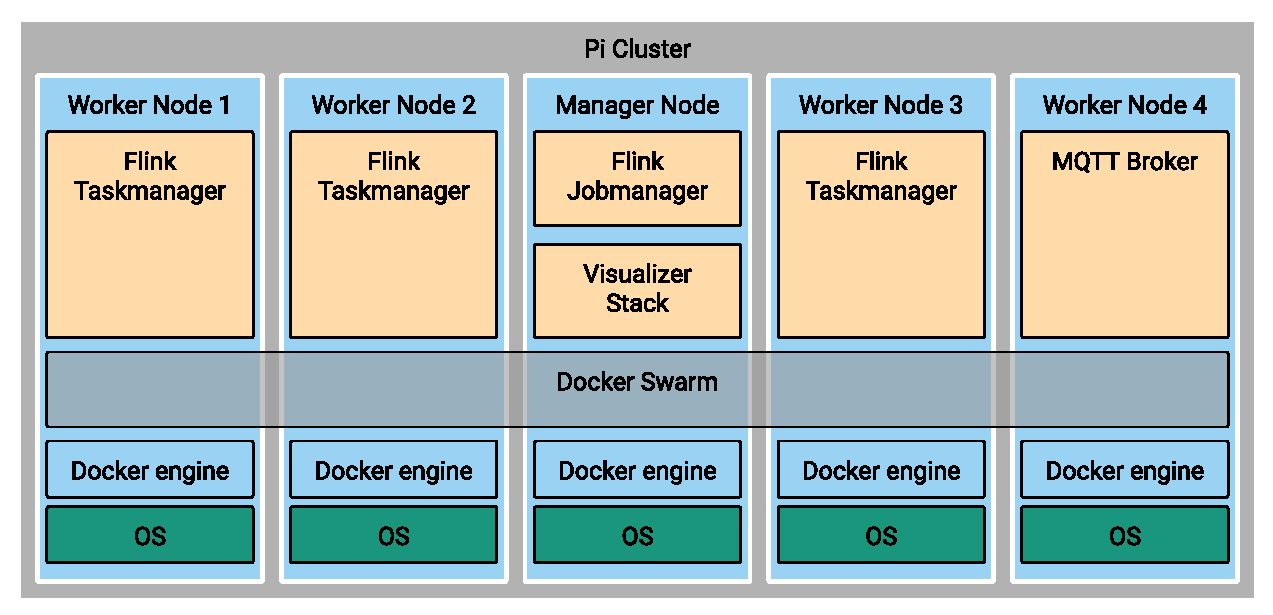
\includegraphics[width=1\linewidth]{figures/fog_platform.pdf}}
\caption{FogGuru: deployment view.}
\label{fig:deployment}
\end{figure}



%%%%%%%%%%%% Demonstration %%%%%%%%%%%%%%%%
\section{Demonstration}
\label{sec:demonstration}
The demonstration setup is depicted in Figure~\ref{fig:demo}. The demonstration mimics a use case in public transportation, whereby data on connected vehicles are collected and aggregated at some fog nodes (which estimate the traffic intensity in a given region).
We use real-world data on connected vehicles, covering $245,369$ vehicles moving across Italy. Data consists of vehicle location, the timestamp of the event created, engine status and type of the vehicle. Events are created converting their recorded timestamp into real-time. On average, $0.8$ events are generated per millisecond.
%DM - taking this out, need to get clearance from Otonomo first
% The raw data is provided by our technology partner Otonomo~\footnote{https://otonomo.io/}.
The processing component implements the following functionality: It filters the incoming traffic by their recorded region and sends aggregated results every 10 seconds to the cloud.
On the cloud tier, we deploy the Telegraf, InfuxDB and Grafana (TIG) stack to receive and visualize aggregated results. The dashboard is shown in Figure~\ref{fig:dashboard}.
% To illustrate the overall architecture and its benefits, we demonstrated the following:
% \paragraph{IoT data generation}
% We simulated IoT traffic using real-life vehicle traffic data recorded throughout Italy.
% \paragraph{Flink Job}
% Processed data pushed every 10 second to custom topic of MQTT broker.
% \paragraph{Monitoring data in a cloud}
% On Cloud environment, we deployed Telegraf, InfuxDB and Grafana (TIG) stack to receive and visualize aggregated results via custom MQTT topic from Fog MQTT broker.
The platform was able to tolerate the traffic without showing any backpressure
while maintaining available processing space for other tasks.


\begin{figure}[htbp]
\centerline{
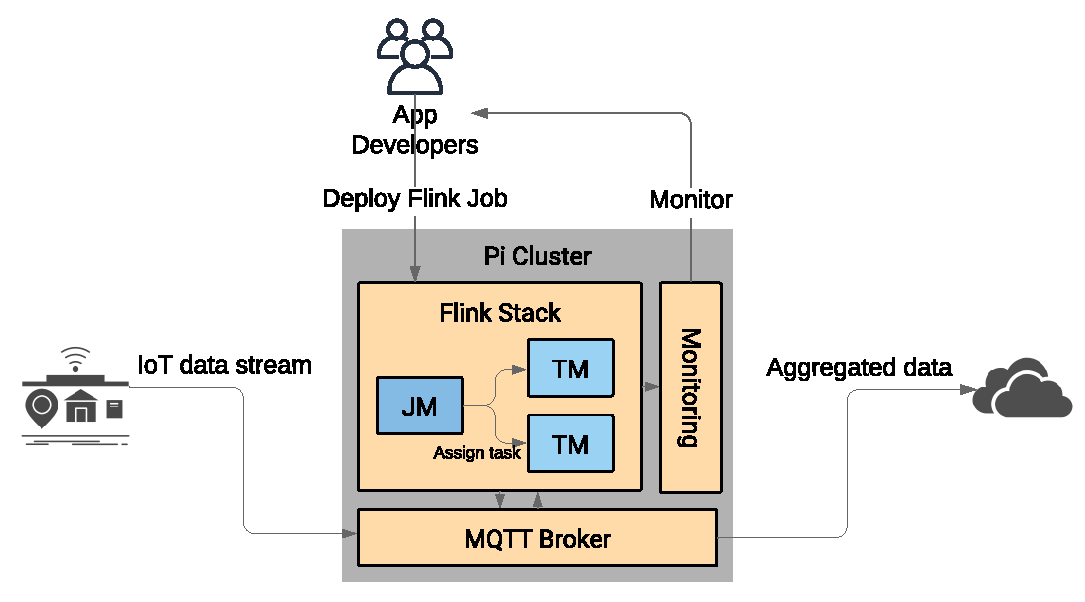
\includegraphics[width=1\linewidth]{figures/fog_activity.pdf}}
\caption{Demonstration setup}
\label{fig:demo}
\end{figure}

\begin{figure}[htbp]
\centerline{
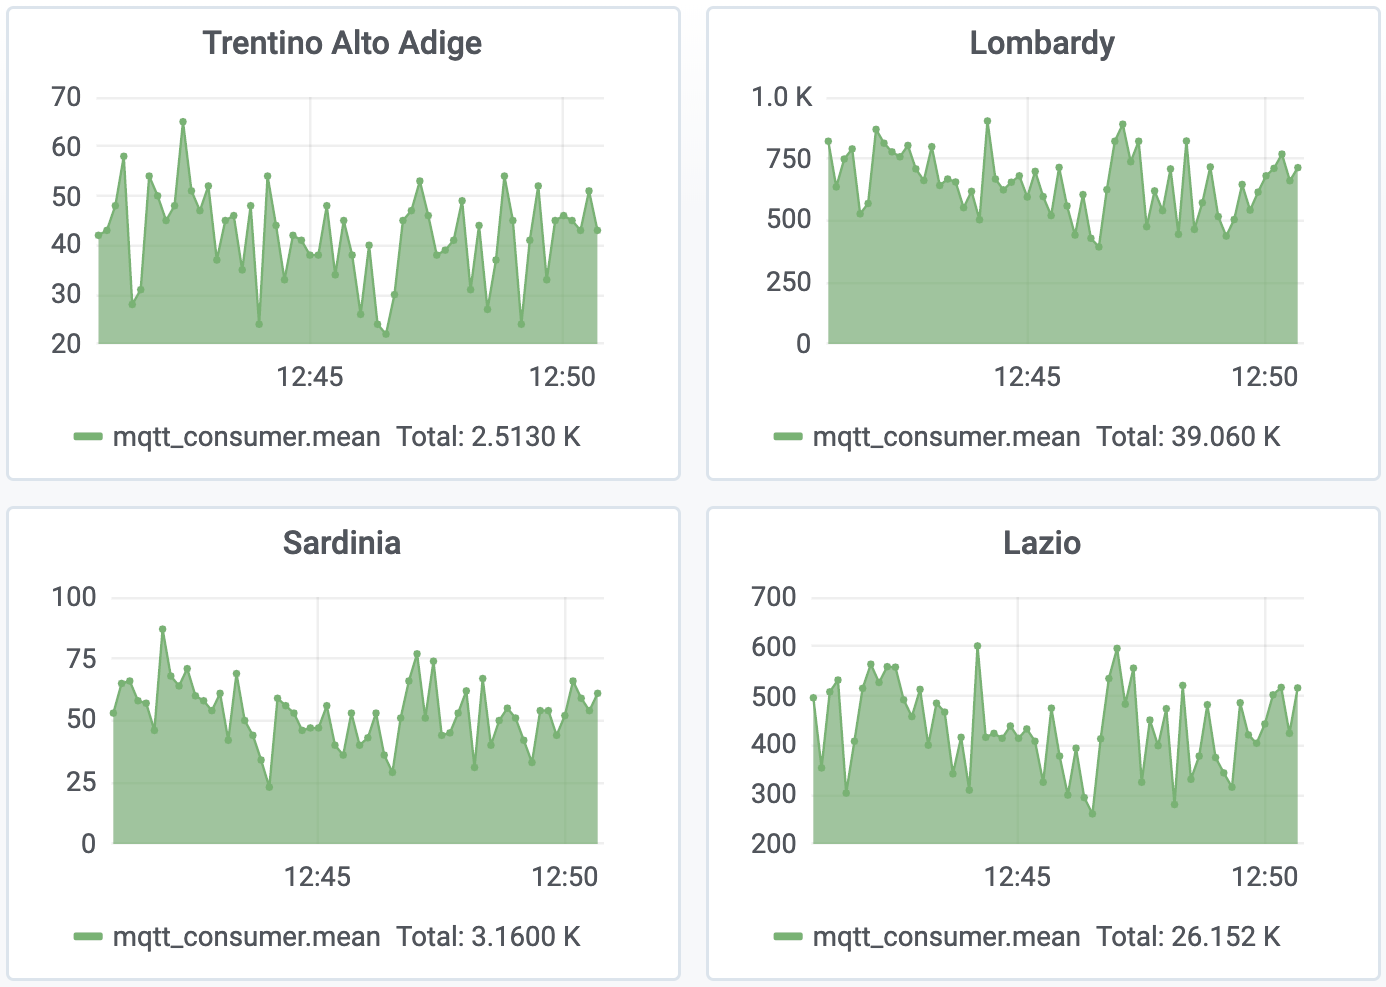
\includegraphics[width=1\linewidth]{figures/fog_dashboard_big.png}}
\caption{Demonstration: the cloud dashboard for traffic monitoring at the regional level.}
\label{fig:dashboard}
\end{figure}





%%%%%%%%%%%% Conclusion and future work %%%%%%%%%%%%%%%%
\section{Conclusion and future work}
\label{sec:conclusion}
In this work, we introduce and demonstrate FogGuru, a platform for developing and deploying fog applications and services based on the stream processing approach. FogGuru was designed to enable applications developers to program fog nodes easily; it is based on a set of open source components implementing open standards. We provide instructions for developers to quickly build and deploy FogGuru on single Raspberry Pis or a cluster thereof (using in the latter case Docker Swarm for orchestrating the deployment).
% This paper presents the design and implementation of a Fog platform based on Apache Flink.
% The re-tasking approach is designed to enhance programmability of Fog platform, taking into account the specifications of application developers.
The demonstration implements a traffic data analytics scenario based on real-world data from 245,369 Internet-connected vehicles. The practical experiments show that the FogGuru prototypical implementation can process in near-time fast data streams from IoT devices.
 % achieved in an acceptable ... .

Future work includes the robust and fault-tolerant deployment of the platform,
integrate autoscaling methods, further devise solutions to automate such
deployments and their continuous optimization, and a more thorough evaluation of
the performance attainable.


\section*{Acknowledgements}

{\small This work is part of the FogGuru project which has received funding from the European Union’s Horizon 2020 research and innovation programme under the Marie Sk\l odowska-Curie grant 765452. The information and views set out
in this publication are those of the author(s) and do not necessarily reflect the official opinion of the European Union. Neither the European Union institutions and bodies nor any person acting on their behalf
may be held responsible for the use which may be made
of the information contained therein.}

{\small The authors thank G. Pierre and colleagues from INRIA in University of Rennes 1
  for assembling the Raspberry Pi cluster.}

% {\small This work is also demonstrated in Flink Forward Berlin in October 2019.}

\bibliographystyle{IEEEtran}
\bibliography{main}


\end{document}
